\section{The area of 3D retrieval} \label{sec:3dretrieval}

With the development of 3D construction techniques, such as new multimedia softwares, interactive tools, 3D scanners and 3D printers, the number of available 3D models on the Internet is increasing. Many domains such as entertainment, medicine, education, and industry field have a growing demand of 3D models, it is much efficient for them to find and reuse a 3D model rather than construct a model which may already exist. This development in 3D field makes the challenges change from construction to retrieval. A basic approach to retrieve data is keyword-based retrieval. However, this simple approach often fails for 3D data. For example, if a 3D model is named as ``1.stl'', both the system and the user can never know its content. Besides, even with keywords, it is difficult to describe a 3D data properly because of the ambiguity in language. 

Therefore, content-based 3D retrieval engines are developed and have been used. Different types of 3D retrieval engines are used in different situations. For example, if the user has an original 3D model and want to find other similar 3D models, the shape-based retrieval system will be helpful~\cite{Funkhouser:2003:SEM:588272.588279}; but if the user has no data to describe what he/she wants to search, and just has an idea about what kind of model does he/she want, sketch-based 3D retrieval will be better~\cite{CGF:CGF12200}. 

\section{Retrieval algorithms} \label{sec:retrievalalgorithms}

Lots of algorithms are developed to describe and match the feature of 3D data. In these algorithms, descriptors are the data that can representing certain features of the model. By extracting one or multiple of these descriptors from two models, matching algorithm can be carried out and determine whether the two data are similar. With reference 3D models (or sketch data), there are many approaches to match them with the candidate models in the database. 

For sketch-based retrieval, one approach is to use 3D sketch as a query to retrieve a similar model, such as the ``Teddy'' by Igarashi~\etal~\cite{Igarashi:2007:TSI:1281500.1281532} and the ``Sketch'' by Zeleznik~\etal~\cite{Zeleznik:2007:SIS:1281500.1281530}. However, the accuracy of the results does not only lie in the robustness of matching algorithms, it also depends on the sketching skill of the user. It is difficult for most users to draw proper sketch for the system to recognize and process. This will increase the processing burden of the system, while make the accuracy of the result decrease. Additionally, the user also need some time to learn to use this kind of drawing interface. 

2D sketches in different views of object are considered as another approach. T. Funkhouser~\etal~\cite{Funkhouser:2003:SEM:588272.588279} provides a solution on 2D sketch based retrieval. In this approach the user only needs to draw 2D projections (usually three orthographic views) of a 3D model. Drawing 2D sketches is easier than 3D sketches, and the interface is much easier for users to learn.  

Recently one another approach by Xie~\etal~\cite{CGF:CGF12200} combines the advantages of the previous 2D and 3D sketches. In their approach the user can draw sketches on the 2D projection of the 3D model, which is interactively updated as the 3D model rotates. It also supports partial object retrieval, and the result can then be combined and assembled to the original object. 

For shape-based 3D retrieval, different approaches focus on exploring different features (descriptors) for object recognition, such as shock graphs~\cite{siddiqi1999shock}, medial axes~\cite{bardinet2000structural}, topology matching~\cite{hilaga2001topology}, skeletons~\cite{sundar2003skeleton}, 3D histogram~\cite{belongie2002shape} and 3D context~\cite{belongie2001matching}. 

3D histogram is one kind of statistical descriptors; it is able to describe the shape context of a 3D object. According to the approach by S. Belongie~\etal~\cite{belongie2001matching}~\cite{belongie2002shape}, the 3D model should be firstly move to its centre of mass. By creating certain voxel grid in space, the number of grids the surface come across is then computed. Therefore the polar histogram in 3D space is created. The advantage of this approach is that the shape context can be easily acquired, and the shape matching can be quickly carried out by searching for shape similarity in the 3D histograms. Also to some extent, the result is robust to noise. However, further processing is required, because the histogram created by this approach will change when the object is rotated. 

Extracting topological information like skeletons is also an approach to carry out shape-based retrieval. H. Sundar~\etal~\cite{sundar2003skeleton} encodes geometric and topological information of 3D models in skeletal graph, so that to measure similarities between 3D models. In this approach firstly transfers the 3D mesh into voxel representations, and then apply an algorithm called Parameter Controlled Volume Thinning by Gagvani~\etal~\cite{gagvani1999parameter}, to acquire the skeletal points. These skeletal points will be connected in an undirected acyclic shape graph. And the graph will be decreased to a denser skeletal graph by minimum spanning tree algorithm. By applying different values of thinness parameter, the hierarchical graph structure can be obtained. The similarities between models are able to be measured by comparing their hierarchical graph structures. 

But these approaches are time-consuming and sensitive to small features. Kazhdan~\etal~\cite{kazhdan2003rotation} uses spherical harmonics to describe shapes and match models. This approach is also applied in a 3D retrieval engine by T. Funkhouser~\cite{Funkhouser:2003:SEM:588272.588279}. The main steps is shown in Figure~\ref{background_sphericalharmonics}. Firstly a voxel grid is created; a binary function is used to represent whether the voxel grid contains the surface of the 3D model.  The results need to be normalized so that to have a unit length from the centre of mass to the average distance from every voxels. These steps make sure the data are scale invariant and high frequency noise can be removed. The next step is to transfer voxels to spherical coordinates so that to obtain the spherical functions. By decomposing the spherical functions, spherical harmonics can be acquired. For each frequency, they add up the harmonics and compute their energy, and then the rotation invariant signature can be acquired. For different radii sum up the different signatures, the spherical harmonics descriptor for 3D data can finally be computed. The result will be a 2D histogram, representing the radius and frequency. Thus it is invariant to rotations. Also because the dimensionality of the descriptor is 2D, this approach will be more efficient in comparing and matching models. And therefore this approach is good for large database. However, its limitation is that it cannot detect models which are different in interior rotation. 

\begin{figure}[h]
\centering
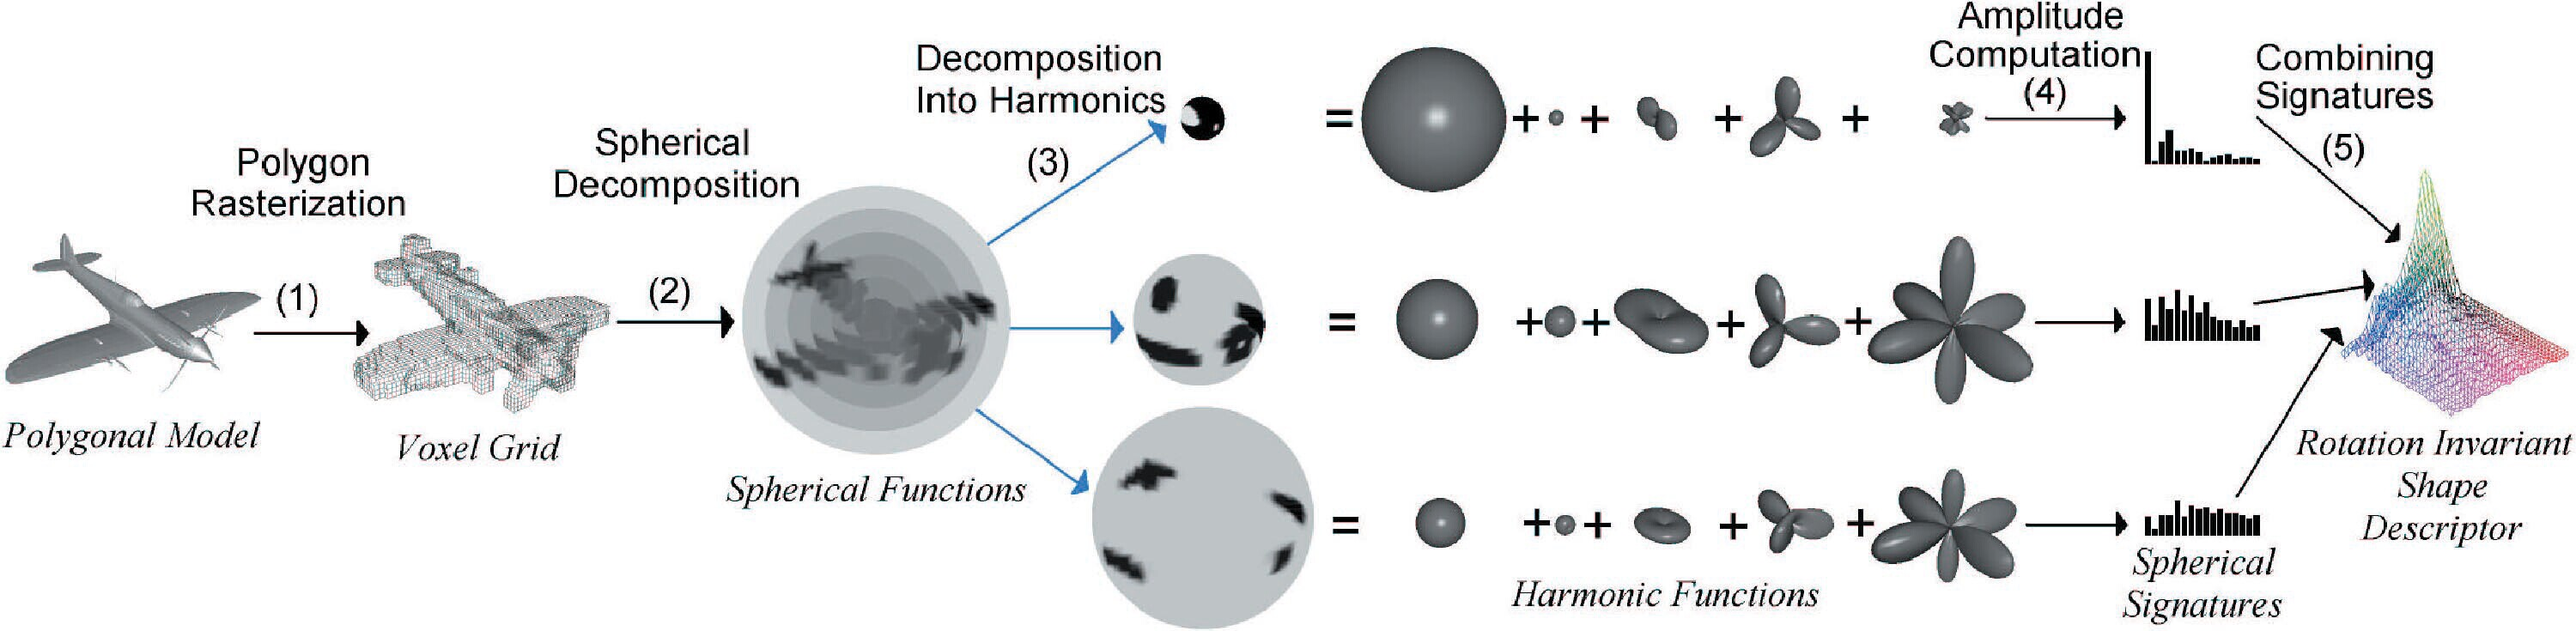
\includegraphics[width=0.9\linewidth]{background_sphericalharmonics}
\caption{Computing spherical harmonics shape descriptor~\cite{Funkhouser:2003:SEM:588272.588279}} \label{background_sphericalharmonics}
\end{figure}


With certain retrieval method, the search engine can be built. Many universities and research institutions have developed their 3D retrieval engines, such as the 3D model search engine at the Princeton University~\cite{shilane2004princeton}~\cite{min2003early}, the 3D model retrieval system at the National Taiwan University~\cite{shen20033d}, and the Purdue University~\cite{iyer2005engineering}. Besides, database and benchmarks are required, for process the search engine as well as testing the search algorithm. The first benchmarks for 3D mesh models is created by Princeton University~\cite{shilane2004princeton}. There are 1, 814 models in the Princeton Shape Benchmark, where half of them are training data and the other half are testing data. In the 3D database of the Purdue University, there are 1,391 models~\cite{iyer2005engineering}.

\section{``Scan to search''} \label{sec:designchoice}

In manufacturing field, many common parts of components has already been designed, and their 3D models have been created. These models have many applications in industrial design and manufacturing. Thus there is no need for some manufactories to recreate these models again - reusing standard parts can lead to reduced production costs. Also with the development of 3D printing techniques, a pre-processed 3D data can directly used for printing and batch producing. Additionally, another situation is that, customers want to find a manufacturing supplier, who can provide certain types of components, they have to look through a list of all kinds of manufacturing components, and choose the right type as well as its suppliers. Or the customer have to be in a meeting with many suppliers, discussing which supplier can produce or provide the certain manufacturing components. It is time-consuming and inefficient, and the customer may miss some suppliers due to the limitation of geography or nationality. 

The company 3DI wants to connect customers and suppliers of manufacturing components through a 3D retrieval system. And this project tries to help 3DI to implement a prototype of shape-based retrieval system, which provides a ``scan to search'' solution. The issue that this system try to solve is, when there is no 3D model data of a component, sketch-based searching cannot provide instant accurate result, and the customer has already had real world sample components, the ``scan to search'' system can provide certain good matching result. The user can scan a object and reconstruct its 3D model, and this system takes the scanned point clouds of manufacturing components as queries, and search for 3D models with similar shape. This is similar to content-based similar image retrieval engine provided by Google. 

To implement this system, there are mainly three parts need to be considered. First is to get the scanned 3D models. An App called ``123D Catch'' will be used. This App can convert a loop of images of an object into a 3D model. Converting from 2D images to 3D model is a challenging topic and it requires lots of efforts to do, and this project is to finish a retrieval system, thus the development of scanning to 3D data will be skipped. Besides, in the early stage, the scanned version of 3D data will be simulated by adding appropriate level of noise. Secondly, models in the database are essential. Since this retrieval system is for searching  manufacturing components, common 3D database is not suitable for testing. Therefore, besides with  Princeton Shape Benchmark~\cite{shilane2004princeton}, many other industrial and manufacturing components are collected from the Internet.

The most important thing for this system is to choose appropriate descriptors. However, before computing descriptors for the scanned 3D model, the noise from scanning should be reduced. Therefore bilateral mesh denoising algorithm~\cite{fleishman2003bilateral} is firstly implemented to remove scanning noise. Considering the input data, even after denoising, they contain unstable shape structure. Besides, the point cloud may lack some important data structures, such as the faces, edges, normal for each vertex information. Due to the unstable structure and remaining scanning noise, some descriptors for shape representing are not suitable, such as the medial axis based descriptors~\cite{kim2001graph} and dihedral angles based descriptors~\cite{gal2009iwires}. These descriptors are sensitive to noise. Besides, skeleton based descriptors~\cite{sundar2003skeleton} is also not suitable. These descriptors would be better for retriving models with similar topological information. For example, humanoid models with a torso and arms and legs, but have different postures. Additionally, since the scanned model cannot be guaranteed to align properly, descriptors should also have rotational invariance property. Therefore, 3D histogram by S. Belongie~\etal~\cite{belongie2002shape}, which is not rotation invariant, cannot be used. Finally, two suitable descriptors can meet the requirements: lightfield descriptors~\cite{shen20033d} and spherical harmonics descriptors~\cite{Funkhouser:2003:SEM:588272.588279}. These two descriptors are both rotation invariant, but spherical harmonics descriptors are more insensitive to noise. Therefore, spherical harmonics descriptors are chosen in this ``scan to search'' retrieval system. 

\section{Computational techniques}
\label{computational_techniques}

\subsection{Spherical harmonics}

In mathematics, spherical harmonics are the angular portion of a set of solutions to Laplace's equation. In computer vision and 3D computer graphics, spherical harmonics are widely used in many topics including lighting (ambient occlusion, global illumination, etc.) and representing the feature of 3D shapes.

The normalized spherical harmonics function can be represented as 
\begin{equation} \label{spherical_harmonics}
Y_\ell^m( \theta , \varphi ) = (-1)^m \sqrt{{(2\ell+1)\over 4\pi}{(\ell-m)!\over (\ell+m)!}} \, P_\ell^m ( \cos{\theta} ) \, e^{i m \varphi },
\end{equation}
where $Y_\ell^m\,\!$ is the spherical harmonics function for $\ell\,\!$ and $m\,\!$. $P_\ell^m\,\!$ is the associated Legendre polynomials. $P_\ell^m\,\!$ can be expressed as 
\begin{equation} \label{legendre}
P_\ell^m(x) = (1 - x^2)^{|m|/2}\ \frac{d^{|m|}}{dx^{|m|}}P_\ell(x)\, .
\end{equation}
$P_\ell(x)\,\!$ is Legendre polynomials on level $\ell\,\!$, which can be represented as Rodrigues' formula:
\begin{equation} \label{rodrigues}
P_\ell(x) = {1 \over 2^\ell \ell!} {d^\ell\over dx^\ell }(x^2 - 1)^l.
\end{equation}

\subsection{Rotation invariant of spherical harmonics}

Spherical harmonics transformation can be applied to any function in spherical coordinates $f(\theta,\varphi)$, and decomposed it as the sum of its harmonics:
\begin{equation} \label{sphericalfunction}
f(\theta,\varphi)=\sum_{l=0}^{\infty}\sum_{m=-l}^{m=l}a_{lm}Y_{l}^{m}(\theta,\varphi),
\end{equation}
where $a_{lm}$ is the coefficient in each frequency. With all the coefficients $a_{lm}$ the spherical function $f(\theta,\varphi)$ can perfectly reconstructed. Therefore, the energy of the sum of the coefficients $a_{lm}$ can represent the feature of the function. 

Let $R()$ denote the rotation, the rotated spherical function is
\begin{equation} \label{rotatedfunction}
R(f(\theta,\varphi))=\sum_{l=0}^{\infty}\sum_{m=-l}^{m=l}=R(a_{lm})Y_{l}^{m}(\theta,\varphi).
\end{equation}
Thus if we compute the $L_{2}$-$norm$ for each coefficient, the energies of a spherical function in each frequency can be acquired as
\begin{equation} \label{l2norm}
\sum_{m=-l}^{m=l}\|a_{ml}\|^{2}=\sum_{m=-l}^{m=l}\|R(a_{ml})\|^{2}.
\end{equation}
The energies do not change if the function is rotated, and thus the results are rotation invariant. Therefore for a 3D model with vertices in polar coordinates, spherical harmonics decomposition can be carried out and the results are unique descriptors that can represent the shape. 

